% TeX compilation engine: XeLaTeX
\documentclass[a4paper,14pt]{extarticle}

% Поля
\usepackage[left=3cm,right=1.5cm,top=2cm,bottom=2cm]{geometry}

% Типографика
\usepackage[russian]{babel}
\usepackage[autostyle=true]{csquotes}
\usepackage{microtype}
\tolerance=1000
\sloppy

% Графика
\usepackage{graphicx}
\usepackage{amssymb}
\usepackage{svg}

% Шрифты
\usepackage{fontspec}
\setmainfont{Times New Roman}

% Интервал
\usepackage{setspace}
\onehalfspacing

% Красная строка
\usepackage{indentfirst}
\setlength{\parindent}{1.25cm} % стандартный абзацный отступ

% Цвет текста
\usepackage{xcolor}
\color{black}

% Создание оглавления
\usepackage{hyperref}
\newcommand{\nosubsection}[1]{%
  \refstepcounter{subsection}%
  \subsection*{\thesubsection\hspace{1em}#1}%
}

% Оглавление на отдельной странице
\usepackage{tocloft}
\renewcommand{\cftsecleader}{\cftdotfill{\cftdotsep}}

% Оформление источников по ГОСТу
\usepackage[style=gost-numeric,sortlocale=ru_RU,natbib=true]{biblatex}
\addbibresource{bibliography.bib}

\begin{document}

\begin{titlepage}
\begin{center}
МИНИСТЕРСТВО НАУКИ И ВЫСШЕГО ОБРАЗОВАНИЯ РОССИЙСКОЙ ФЕДЕРАЦИИ\\
Федеральное государственное автономное образовательное учреждение высшего образования\\
\textbf{«Национальный исследовательский Нижегородский государственный университет им. Н.И. Лобачевского» (ННГУ)}\\
\vspace*{\fill}
{\LARGE Новая концепция интеграла,\\предложенная Лебегом, и ее развитие}\\
\vspace{2cm}
\end{center}
\hfill
\begin{minipage}{0.4\textwidth}
\raggedright
\textbf{Выполнил:}\\
Власов Максим Сергеевич,\\
студент группы 3823М1ПМкн\\
\end{minipage}
\vspace*{\fill}
\begin{center}
Нижний Новгород\\
2024
\end{center}
\end{titlepage}

\newpage
\setcounter{page}{2}
\tableofcontents

\newpage
\section*{Введение}
\addcontentsline{toc}{section}{Введение}

Интегральное исчисление -- одна из фундаментальных областей математического анализа, которая играет важнейшую роль как в теоретической математике, так и в ее приложениях. Понятие интеграла возникает при решении задач о нахождении площади под кривой, пройденного пути при неравномерном движении, массы неоднородного тела и тому подобных, а также в задаче о восстановлении функции по её производной. 

На протяжении столетий математиков устраивало интегрирование в рамках концепции, предложенной Риманом, однако развитие науки и появление более сложных задач выявили ограничения этого подхода. Например, интеграл Римана не справляется с функциями, имеющими сложные множества точек разрыва или функции, определенные на бесконечных множествах с особенностями.

В начале XX века французский математик Анри Лебег предложил новую концепцию интеграла, основанную на разбиении области значений функции вместо области определения. Эта идея не только позволила интегрировать более широкий класс функций, но и значительно обогатила математический анализ. Интеграл Лебега стал основой для новых областей исследований, таких как теория меры и функциональный анализ, а также получил применение в теории вероятностей, физике и статистике.

Целью данного реферата является рассмотрение концепции интеграла Лебега, анализ его преимуществ перед интегралом Римана и изучение развития этой теории в последующих работах. В работе также будут представлены ключевые применения интеграла Лебега в различных научных областях.

\newpage
\section{Интеграл Римана}

Интеграл Римана -- наиболее широко используемый вид определённого интеграла. Очень часто под термином «определённый интеграл» понимается именно интеграл Римана, и он изучается самым первым из всех определённых интегралов во всех курсах математического анализа. Введён Бернхардом Риманом в 1854 году, и является одной из первых формализаций понятия интеграла. ~\cite{wikipedia_riemann_integral}

Интеграл Римана есть формализация понятия площади под графиком некоторой функции $f(x)$. Разобьём отрезок $[a; b]$, над которым мы ищем площадь, на конечное число подотрезков. На каждом из подотрезков выберем некоторую точку графика $\xi_i$ и построим вертикальный прямоугольник с подотрезком в качестве основания до той самой точки графика. Рассмотрим фигуру, полученную из таких прямоугольников, называемую криволинейной трапецией.

\begin{figure}[h]
    \centering
    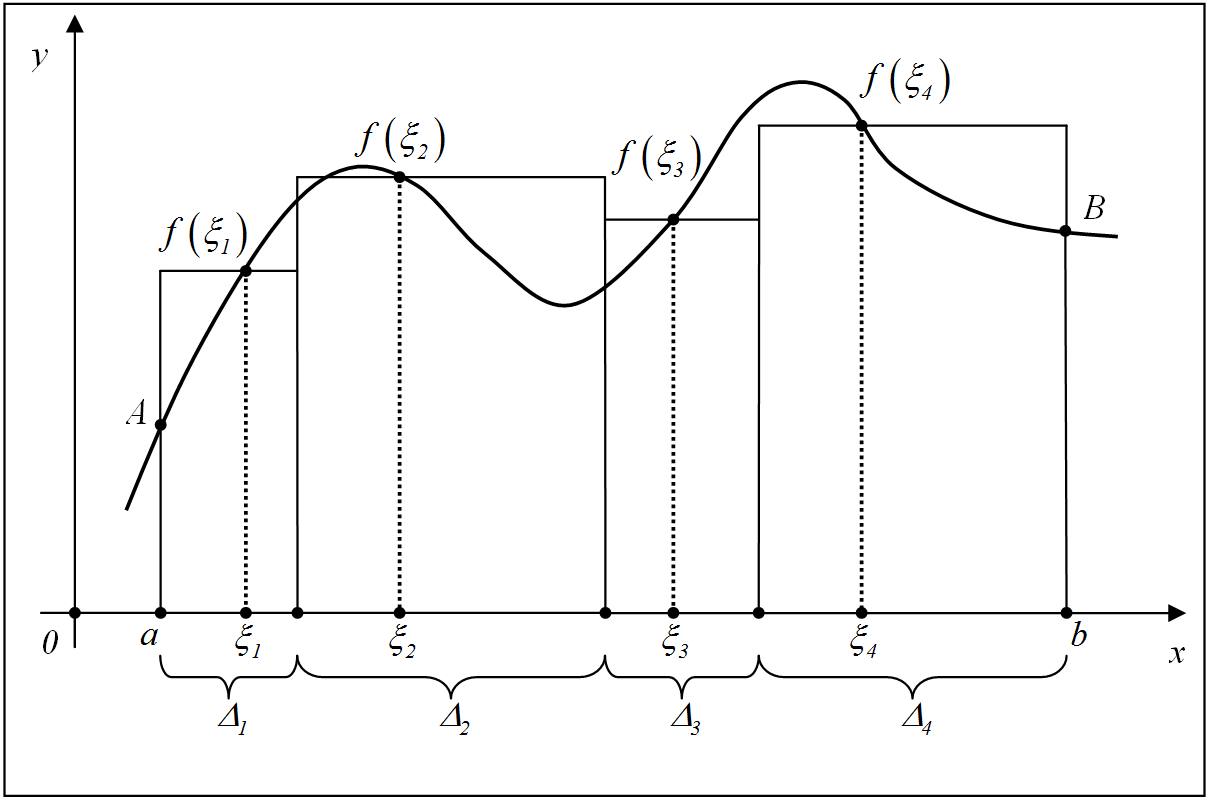
\includegraphics[width=0.75\textwidth]{images/riemann_integral.png}
    \caption{Пример вычисления суммы по Риману.}
\end{figure}

Площадь $S$ такой фигуры при конкретном разбиении на отрезки длинами $\Delta x_i$ будет задаваться суммой:

$$
\sigma = \sum_i f(x_i) \Delta x_i
$$

Интуитивно понятно, что если мы будем уменьшать длины этих подотрезков ($\max \Delta x_i \rightarrow 0$), то площадь такой фигуры будет всё больше и больше приближаться к площади под графиком. Именно это замечание и приводит к определению интеграла Римана. ~\cite{fichtenholz}

Таким образом, если существует, независимо от выбора точек разбиения отрезка и точек $\xi_i$, предел суммы $\sigma$ при стремлении длин всех отрезков к нулю, то такой предел называется определённым интегралом Римана от функции $f(x)$ по отрезку $[a; b]$ и обозначается

$$
\int\limits_a^b f(x) dx.
$$

Сама функция при этом называется интегрируемой на отрезке $[a; b]$. Суммы $\sigma$ называются интегральными суммами.

Интеграл по Риману применим к функциям, которые определены на конечном отрезке и ограничены на нем. Допускаются точки разрыва, но они должны образовывать множество нулевой меры (то есть их совокупная «длина» должна быть равна нулю, как, например у функций с конечным числом разрывов на отрезке или с разрывами в счетном наборе точек).

Однако интеграл не может быть определен для некоторых функций, разрывных на бесконечном множестве точек, даже если эти точки образуют множество с нулевой мерой. Также интеграл Римана плохо справляется с задачами, где нужно изучать предел последовательности функций. Например, при переходе к пределу последовательности функций может «потеряться» их интегрируемость. Неформально, интеграл Римана ограничен областью определения функций, которые можно разбить на стандартные интервалы. Он не может работать с функциями, определенными на более сложных множествах (например, на бесконечных множествах, как Канторово множество).

\newpage
\section{Интеграл Лебега}

Интеграл Лебега был разработан для преодоления ограничений применимости интеграла Римана. Его основной целью было расширение понятия интегрируемости на более широкий класс функций и возможность работы с функциями, определенными на произвольных множествах. Это стало возможным благодаря новому подходу к интегрированию, предложенному французским математиком Анри Лебегом.

Для вычисления интеграла Римана функции $f$ интервал $[a, b]$ делится на подинтервалы, в то время как в случае с интегралом Лебега фактически происходит разбиение области значений функции $f$. Для определения введем понятие меры Лебега $\mu$. В самом простом случае мера $\mu(A)$ для интервала $A = [a, b]$ равна его длине $b - a$, так что интеграл Лебега совпадает с (собственным) интегралом Римана, когда оба существуют. В более сложных случаях измеримые множества могут не быть непрерывными и вообще не иметь сходства с интервалами.

\begin{figure}[h]
    \centering
    \includesvg[width=0.75\textwidth]{images/lebesgue_integral.svg}
    \caption{Приближение интеграла по Лебегу.}
\end{figure}

Используя подход «разбиения области значений функции $f$», интеграл неотрицательной измеримой функции $f : \mathbb{R} \to \mathbb{R}$ по Лебегу должен быть суммой по $t$ мер между тонкими горизонтальными полосами, ограниченными $y = t$ и $y = t + dt$. Эта мера равна $\mu (\{x : f(x) > t\}) \, dt$. Пусть

$$
f^*(t) = \mu(\{x : f(x) > t\}).
$$

Тогда Лебегов интеграл функции $f$ определяется как

$$
\int\limits_a^b f(x) d\mu = \int_0^\infty f^*(t)\,dt
$$

\noindent где интеграл справа — это несобственный интеграл Римана (так как $f^*(t)$ — строго убывающая положительная функция). ~\cite{wikipedia_lebesgue_integral}

Интеграл Лебега обладает всеми хорошими свойствами обычного интеграла, а именно, интеграл от суммы равен сумме интегралов, постоянный множитель можно выносить за знак интеграла и т. д. Однако интеграл Лебега обладает еще одним замечательным свойством, которым интеграл Римана не обладает: если измеримые функции $f_n(x)$ ограничены в совокупности: $|f_n(x)| < K$ для любого $n$ и любого $x$ из отрезка $[a; b]$ и последовательность $\{f_n(x)\}$ сходится почти всюду к функции $f(x)$, то

$$
\int\limits_{a}^{b}f_n(x)\,dx\to\int\limits_{a}^{b}f(x)\,dx.
$$

Иными словами, интеграл Лебега допускает безотказный переход к пределу. Именно это свойство интеграла Лебега делает его весьма удобным, а часто и неизбежным инструментом во многих исследованиях. В частности, интеграл Лебега совершенно необходим в теории тригонометрических рядов, в теории функциональных пространств и других разделах математики. ~\cite{mathhelpplanet_lebesgue_integral}

Можно выделить следующие основные преимущества идеи интегрирования по Лебегу по сравнению с интегралом Римана:

\begin{itemize}
    \item \textbf{Более широкий класс интегрируемых функций.} Интеграл Лебега позволяет интегрировать, например, функции с разрывами на множествах с положительной мерой или функции, которые не имеют явных ограничений по непрерывности и не интегрируемы по Риману.
    \item \textbf{Удобство для работы с пределами функций.} Теоремы о сходимости (монотонной и мажорированной) позволяют безопасно выносить операторы предела и интеграла при выполнении преобразований формул, что важно при работе с последовательностями функций, например, в приложениях анализа, при рассмотрении предельных процессов в функциональном анализе и теории вероятностей.
    \item \textbf{Обработка разрывных функций.} Интеграл Лебега позволяет корректно работать с функциями, которые могут иметь разрывы на множествах с положительной мерой. В отличие от интеграла Римана, который ограничен функциями с разрывами на множествах меры ноль, интеграл Лебега может интегрировать функции, разрывы которых расположены на множестве, имеющем положительную меру, что делает его более универсальным инструментом.
    \item \textbf{Интеграция по произвольным множествам.} Интеграл Лебега основывается на теории меры, что позволяет интегрировать функции, определенные на произвольных множествах, а не только на отрезках или интервалах. Это делает его удобным инструментом для работы с более сложными множествами, включая такие объекты, как Броуновское движение или другие случайные процессы, которые требуют работы с более сложными структурами.
    \item \textbf{Гибкость при преобразованиях функций.} Интеграл Лебега устойчив к различным преобразованиям функций, таким как сжатие или растяжение.
\end{itemize}

Эти преимущества делают интеграл Лебега более универсальным и мощным инструментом для математического анализа и его приложений. ~\cite{folland}

Рассмотрим функцию Дирихле $D(x) \equiv \chi_{\mathbb{Q}_{[0,1]}}(x)$, заданную на $[0; 1]$ с мерой Лебега $\mu$. Эта функция принимает значение $1$ в рациональных точках и $0$ в иррациональных. Легко увидеть, что $D$ не интегрируема в смысле Римана. Однако она является простой функцией на пространстве с конечной мерой, так как принимает только два значения, и её интеграл Лебега определён и равен:

$$
\int\limits_{[0,1]} D(x)\, \mu(dx) = 1 \cdot \mu(\mathbb{Q}_{[0,1]}) + 0 \cdot \mu([0,1] \setminus \mathbb{Q}_{[0,1]}) = 1 \cdot 0 + 0 \cdot 1 = 0.
$$

Действительно, мера отрезка $[0; 1]$ равна $1$, и так как множество рациональных чисел счётно, то его мера равна $0$, а значит мера иррациональных чисел равна $1 - 0 = 1$.

\newpage
\section{Приложения интеграла Лебега}

Интеграл Лебега является мощным инструментом в математике, используемым в различных областях. Он расширяет понятие интегрирования, что позволяет работать с более общими функциями и пределами. Рассмотрим его применение в некоторых основных разделах математики.

\nosubsection{Функциональный анализ}

Интеграл Лебега играет ключевую роль в функциональном анализе, где он используется для определения и изучения пространств Лебега $L^p$. Эти пространства состоят из функций, для которых $p$-я степень абсолютного значения интеграбельна:

$$
L^p(X, \mu) = \left\{ f: X \to \mathbb{R} \mid \int_X |f|^p \, d\mu < \infty \right\}.
$$

\noindent Здесь интеграл Лебега позволяет работать с функциями, которые не обязательно непрерывны, что расширяет спектр исследуемых задач.

\nosubsection{Вероятность и статистика}

В теории вероятностей интеграл Лебега используется для работы с распределениями вероятностей. Здесь он упрощает вычисления, особенно когда случайные величины имеют сложные распределения. Ожидания и моменты случайных величин можно выразить через интеграл Лебега, что является особенно полезным в изучении пределов распределений и законе больших чисел:

$$
\mathbb{E}[X] = \int_\Omega X \, d\mathbb{P},
$$

\noindent где $\mathbb{P}$ — мера вероятности.

\nosubsection{Теория дифференциальных уравнений}

При изучении дифференциальных уравнений, особенно в нелинейных контекстах, интеграл Лебега применяется для определения слабых решений и работ с обобщенными функциями. Он позволяет обобщить понятие производной и интеграла, что необходимо в тех случаях, когда классические решения могут не существовать.

Слабые решения часто определяются на основе функционалов Лебега:

$$
\int \phi(x) f'(x) \, dx = -\int \phi'(x) f(x) \, dx,
$$

\noindent где $\phi$ — тестовая функция.

\nosubsection{Гармонический анализ}

В гармоническом анализе интеграл Лебега используется для работы с преобразованиями Фурье и другими инструментами, которые требуют анализа функций высокой степени обобщенности. В этом контексте важными являются теоремы о сближении, такие как теорема Леви о мажорантной сходимости и теорема о предельной сходимости, которые дают условия, при которых можно менять порядок пределов и интегралов:

$$
\lim_{n \to \infty} \int f_n \, d\mu = \int \lim_{n \to \infty} f_n \, d\mu,
$$

\noindent где сходимость и интегрируемость обосновываются условиями из теоремы.

\nosubsection{Физика}

В квантовой механике интеграл Лебега применяется для вычисления вероятностных амплитуд и нормировок волновых функций. Поскольку пространственные распределения вероятностей в квантовых системах могут быть разрывными или даже сингулярными\footnote{Сингулярная функция -- это непрерывная функция, производная которой равна нулю почти всюду.}, интеграл Лебега обеспечивает корректные вычисления. Например, нормировка волновой функции $\psi(x)$ требует, чтобы интеграл вероятности равнялся единице:

$$
\int |\psi(x)|^2 \, dx = 1.
$$

Для пространства с дискретным и непрерывным спектром можно использовать интеграл Лебега для более общей нормировки, особенно когда функции волнового пакета делят спектральное пространство на множество подмножеств с разной мерой.

Интеграл Лебега полезен и в статистической механике, особенно при интегрировании сложных функций распределения, как, например, плотность состояний. Для системы с большим числом степеней свободы, функции распределения могут быть сингулярными на отдельных участках фазового пространства, и применение интеграла Лебега обеспечивает полноту интерпретации, позволяя точные вычисления равновесных свойств.

Таким образом, интеграл Лебега -- это универсальный инструмент, который находит применение в различных разделах математики, обобщает классические методы и решает более сложные проблемы, чем это возможно при использовании интеграла Римана. Также благодаря своей способности корректно интегрировать сложные, разрывные и сингулярные функции, интеграл Лебега находит широкое приложение в различных разделах физики для исследования сложных систем, особенно в контексте статистических моделей и моделей квантовой механики.

\newpage
\section{Интеграл Лебега-Стильтеса}

Интеграл Лебега-Стильтеса представляет собой обобщение интегралов Лебега и Римана, которое позволяет интегрировать не относительно длины (меры в интеграле Лебега), а относительно произвольной функции монотонного изменения $g(x)$. Этот интеграл полезен в различных областях математики, включая теорию вероятностей и финансовую математику, где для моделирования применяются распределения и плотности, описанные функциями распределения, которые могут быть дискретными, непрерывными или смешанными.

Пусть $f : [a, b] \to \mathbb{R}$ — измеримая функция и $g : [a, b] \to \mathbb{R}$ — монотонная функция. Интеграл Лебега-Стильтеса функции $f$ относительно функции $g$ на промежутке \([a, b]\) можно обозначить как:

$$
\int_a^b f(x) \, dg(x).
$$

Интеграл Лебега-Стильтеса играет важную роль в теории вероятностей, особенно в контексте случайных процессов и ожидаемых значений. Например, если $X$ — случайная величина с функцией распределения $F(x)$, то математическое ожидание функции от этой случайной величины, скажем, $f(X)$, может быть выражено как:

$$
\mathbb{E}[f(X)] = \int_{-\infty}^{\infty} f(x) \, dF(x).
$$

Рассмотрим случай, когда $f(x) = x$ и $g(x)$ — функция распределения случайной величины. В этом случае интеграл Лебега-Стильтеса даёт нам ожидаемое значение случайной величины $X$:

$$
\mathbb{E}[X] = \int_{-\infty}^{\infty} x \, dF(x).
$$

Таким образом, интеграл Лебега-Стильтеса предлагает обобщённое и гибкое перспективное средство для интегрирования, особенно полезное в случаях, где используются функции распределения или меры, отличные от стандартных. ~\cite{wikipedia_lebesgue_stieltjes}

\newpage
\section*{Заключение}
\addcontentsline{toc}{section}{Заключение}

Концепция интеграла Лебега значительно расширила возможности математического анализа, преодолев ограничения традиционного интеграла Римана. В то время как интеграл Римана был эффективным инструментом для работы с непрерывными и ограниченными функциями, его возможности оказались ограниченными в случае более сложных сущностей, таких как функции с разрывами на множествах с положительной мерой или функции, определенные на сложных множествах. Интеграл Лебега, основанный на теории меры, решает эти проблемы, предоставляя возможность интегрировать более широкий класс функций, включая функции с разрывами на множестве неограниченного размера и даже на множествах, имеющих более сложную структуру, чем интервалы.

Благодаря новым подходам, таким как разбиение области значений функции и использование меры, интеграл Лебега стал основой для развития множества важных теорий в математике, включая функциональный анализ, теорию вероятностей, статистику и квантовую механику. Применение интеграла Лебега позволило решать более сложные задачи, такие как исследование пределов интегралов, обработка последовательностей функций и расширение интеграции на произвольные множества.

В дальнейшем развитие интеграла Лебега привело к созданию еще более обобщенных интегралов, таких как интеграл Лебега-Стилтьеса, что открыло новые горизонты для исследований в математике и смежных областях. Поэтому интеграл Лебега остается важным инструментом как для теоретического анализа, так и для практических приложений в самых различных областях науки.

\newpage
\addcontentsline{toc}{section}{Список литературы}
\printbibliography

\end{document}
